\documentclass[11pt,a4paper]{article}

% Packages
\usepackage[margin=2.3cm]{geometry}
\usepackage{microtype}
\usepackage{graphicx}
\usepackage{tikz}
\usetikzlibrary{shapes,arrows.meta,positioning,calc,fit,backgrounds,shadows.blur,decorations.pathmorphing,decorations.pathreplacing}
\usepackage{colortbl}
\usepackage{enumitem}
\usepackage{booktabs}
\usepackage{longtable}
\usepackage{array}
\usepackage{hyperref}
\usepackage{xcolor}
\usepackage{fancyhdr}
\usepackage{titlesec}
\usepackage[most]{tcolorbox}
\usepackage{amsmath,amssymb}
\usepackage{setspace}
\usepackage{fontawesome5}
\usepackage{listings}

% Spacing
\setlength{\parskip}{3pt plus 1pt minus 1pt}
\setlength{\parindent}{0pt}
\renewcommand{\arraystretch}{1.25}

% Colors
\definecolor{primary}{HTML}{1A5276}
\definecolor{secondary}{HTML}{2E86C1}
\definecolor{accent}{HTML}{E74C3C}
\definecolor{lightbg}{HTML}{EBF5FB}
\definecolor{defbg}{HTML}{FDF2E9}
\definecolor{greenhl}{HTML}{27AE60}
\definecolor{purplehl}{HTML}{8E44AD}
\definecolor{codebg}{HTML}{F4F6F7}

% Hyperref
\hypersetup{colorlinks=true, linkcolor=primary, urlcolor=secondary, citecolor=primary}

% Code listings style
\lstset{
  backgroundcolor=\color{codebg},
  basicstyle=\ttfamily\small,
  keywordstyle=\color{primary}\bfseries,
  stringstyle=\color{greenhl},
  commentstyle=\color{gray},
  breaklines=true,
  frame=l,
  framerule=2pt,
  rulecolor=\color{secondary!40},
  xleftmargin=8pt,
  framexleftmargin=6pt,
  aboveskip=6pt,
  belowskip=6pt,
  showstringspaces=false,
  language=Python
}

% Header/Footer
\pagestyle{fancy}
\fancyhf{}
\fancyhead[L]{\small\textcolor{primary}{\textbf{Data Science --- Midterm Answer Key}}}
\fancyhead[R]{\small\textcolor{primary}{BSIT}}
\fancyfoot[C]{\small\thepage}
\renewcommand{\headrulewidth}{0.5pt}
\renewcommand{\footrulewidth}{0.3pt}

% Section formatting
\titleformat{\section}{\large\bfseries\color{primary}}{}{0em}{}[\vspace{2pt}\titlerule]
\titlespacing*{\section}{0pt}{14pt}{8pt}

% Custom boxes
\newtcolorbox{definitionbox}[1][]{
  enhanced, breakable,
  colback=defbg, colframe=orange!60!black,
  colbacktitle=orange!70!black, coltitle=white,
  title={\faIcon{book}~#1}, fonttitle=\bfseries,
  boxrule=0pt, leftrule=4pt, arc=2pt,
  shadow={1mm}{-1mm}{0mm}{black!15},
  top=4pt, bottom=4pt, left=8pt, right=8pt
}
\newtcolorbox{conceptbox}[1][]{
  enhanced, breakable,
  colback=lightbg, colframe=secondary,
  colbacktitle=secondary, coltitle=white,
  title={\faIcon{lightbulb}~#1}, fonttitle=\bfseries,
  boxrule=0pt, leftrule=4pt, arc=2pt,
  shadow={1mm}{-1mm}{0mm}{black!15},
  top=4pt, bottom=4pt, left=8pt, right=8pt
}

% Question header box
\newtcolorbox{qbox}[1][]{
  enhanced, breakable,
  colback=primary!8, colframe=primary,
  boxrule=0pt, leftrule=4pt, arc=2pt,
  top=4pt, bottom=4pt, left=8pt, right=8pt,
  fontupper=\bfseries
}

\newcommand{\question}[2]{%
  \begin{qbox}#1\hfill\textcolor{accent}{(05 marks)}\\[2pt]#2\end{qbox}%
}

\begin{document}

% Title
\begin{center}
\vspace*{0.3cm}
{\Huge\bfseries\textcolor{primary}{Midterm Answer Key}}\\[8pt]
{\Large\bfseries\textcolor{primary}{Data Science, AI \& Emerging Paradigms}}\\[14pt]
{\color{secondary}\rule{0.6\textwidth}{1.5pt}}\\[12pt]
{\Large\textsc{BSIT --- Data Science}}\\[6pt]
{\large\textcolor{gray!70!black}{Concise, To-the-Point Answers Extracted from Course Handouts}}
\vspace{0.2cm}
\end{center}

%=============================================================
\question{Q-1. How do bagging, boosting, and stacking differ?}{}

Bagging, boosting, and stacking are the three main \textbf{ensemble} techniques that combine multiple models to improve performance.

\begin{center}
\begin{tabular}{@{}>{\bfseries}p{2.4cm}p{3.6cm}p{3.6cm}p{4.4cm}@{}}
\toprule
\rowcolor{primary!15}
\textbf{Aspect} & \textbf{Bagging} & \textbf{Boosting} & \textbf{Stacking} \\
\midrule
Core idea & Train models in parallel on varied bootstrap samples & Train models sequentially; each focuses on earlier errors & Combine outputs of several models using a meta-model \\
How models train & Independently, in parallel & Dependently, one after another & Base models trained, then a meta-learner on their outputs \\
Data used & Random subsets (with replacement) & Full data, re-weighting hard cases & Predictions of base models as new features \\
Main effect & Reduces variance & Reduces bias (and variance) & Reduces both by blending diverse models \\
Combination & Majority vote / averaging (equal weight) & Weighted by model performance & Learned by the meta-model \\
Overfitting & Less prone to overfitting & Can overfit if not regularized & Depends on base/meta models \\
Examples & Random Forest & AdaBoost, Gradient Boosting, XGBoost, LightGBM, CatBoost & Stacked generalization with a meta-learner \\
\bottomrule
\end{tabular}
\end{center}

%=============================================================
\question{Q-2. Compare Generative AI vs. Agentic AI.}{}

\begin{center}
\begin{tabular}{@{}>{\bfseries}p{3.0cm}p{5.2cm}p{5.2cm}@{}}
\toprule
\rowcolor{primary!15}
\textbf{Aspect} & \textbf{Generative AI} & \textbf{Agentic AI} \\
\midrule
Primary focus & Content generation & Goal-driven action \\
Core capability & Generate text, images, code, or audio & Decide, plan, and act \\
Autonomy & Often limited & Higher and more persistent \\
Interaction style & Prompt-based & Environment-based or tool-based \\
Memory & Often short-term & Often persistent or state-aware \\
Typical output & Content & Actions, plans, decisions, and content \\
\bottomrule
\end{tabular}
\end{center}

\begin{conceptbox}[Integration Principle]
Generative AI often acts as the cognitive engine inside an agentic system, while agentic AI adds planning logic, tools, memory, and goal management around that engine.
\end{conceptbox}

%=============================================================
\question{Q-3. Main purposes of GitHub Copilot Ask, Edit, and Agent modes.}{}

\begin{center}
\begin{tabular}{@{}>{\bfseries}p{2.4cm}p{4.6cm}p{6.4cm}@{}}
\toprule
\rowcolor{primary!15}
\textbf{Mode} & \textbf{What It Does} & \textbf{Typical Use} \\
\midrule
Ask mode & Answers questions, explains code, suggests approaches & Learn concepts, debug errors, understand algorithms, ask for examples \\
Edit mode & Applies requested changes to code or text & Refactor functions, update notebooks, fix formatting, rewrite blocks \\
Agent mode & Works through a multi-step task using repo context and tools & Search files, update several places, run validations, complete coding tasks \\
\bottomrule
\end{tabular}
\end{center}

\begin{conceptbox}[How to Choose]
Use \textbf{Ask} to understand topics before copying code, \textbf{Edit} when you already know what you want changed, and \textbf{Agent} for larger tasks that involve multiple steps or files.
\end{conceptbox}

%=============================================================
\question{Q-4. Compare AI Agent vs. Chatbot vs. Traditional Automation.}{}

\begin{center}
\begin{tabular}{@{}>{\bfseries}p{3.0cm}p{3.6cm}p{3.4cm}p{3.4cm}@{}}
\toprule
\rowcolor{primary!15}
\textbf{System} & \textbf{Main Behavior} & \textbf{Strength} & \textbf{Limitation} \\
\midrule
Basic chatbot & Answers direct questions & Easy to use & Usually limited to one-turn responses \\
Traditional automation & Follows fixed rules or scripts & Reliable for repeated tasks & Cannot adapt well to new situations \\
AI agent & Plans, acts, checks results, and continues & More flexible and capable & Needs guardrails and monitoring \\
\bottomrule
\end{tabular}
\end{center}

\begin{conceptbox}[Key Difference]
A chatbot mainly \textbf{responds}. An AI agent can \textbf{respond, decide, act, observe, and continue working}.
\end{conceptbox}

%=============================================================
\question{Q-5. How does a data scientist proceed from a real problem to a data science task?}{}

A real-world goal is \textbf{translated (formulated) into a concrete data science task} with a clear target and a measurable success metric, then constraints are balanced.

\begin{center}
\begin{tabular}{@{}p{4.0cm}p{4.0cm}p{5.0cm}@{}}
\toprule
\rowcolor{primary!15}
\textbf{Real-World Goal} & \textbf{Data Science Formulation} & \textbf{Possible Metrics} \\
\midrule
Identify at-risk students & Binary classification & Recall, precision, F1-score, calibration \\
Forecast course enrollment & Time series forecasting & MAE, RMSE, MAPE \\
Recommend learning materials & Ranking or recommendation & Precision@k, Recall@k, NDCG \\
Detect unusual student system behavior & Anomaly detection & Detection rate, false alarm rate \\
\bottomrule
\end{tabular}
\end{center}

\textbf{Then define success criteria and tradeoffs:}
\begin{itemize}[leftmargin=*,topsep=2pt]
  \item \textbf{Offline metrics:} Accuracy, RMSE, F1-score, AUC, ranking metrics.
  \item \textbf{Operational metrics:} Latency, throughput, availability, compute cost.
  \item \textbf{Business/institutional metrics:} Retention rate, intervention success, decision quality.
  \item \textbf{Safety and governance metrics:} Bias, drift, privacy compliance, reviewability.
\end{itemize}

\begin{conceptbox}[Why It Matters]
Real systems rarely optimize only one thing. If the project question, metric, user, or decision context is unclear, even a technically strong model may create little value.
\end{conceptbox}

%=============================================================
\question{Q-6. Explain when deep learning is a good choice.}{}

\begin{center}
\begin{tabular}{@{}p{6.5cm}p{6.5cm}@{}}
\toprule
\rowcolor{primary!15}
\textbf{Deep Learning Often Fits Well} & \textbf{Traditional ML May Be Better First} \\
\midrule
Large image, audio, or text datasets & Small datasets with limited samples \\
Very complex relationships in the data & Problems where high interpretability is required \\
Tasks where automatic feature learning helps & Cases where a simple model already works well \\
Applications that can use GPU acceleration & Projects with very limited computing resources \\
\bottomrule
\end{tabular}
\end{center}

\begin{conceptbox}[Important Note]
Deep learning is not always the best first model. In many business and classroom projects, a simpler method such as logistic regression, decision trees, or random forests may be easier to train, explain, and deploy.
\end{conceptbox}

%=============================================================
\question{Q-7. What is the difference between a parameter and a hyperparameter?}{}

\begin{center}
\begin{tabular}{@{}>{\bfseries}p{3.0cm}p{5.0cm}p{5.0cm}@{}}
\toprule
\rowcolor{primary!15}
\textbf{Aspect} & \textbf{Parameter} & \textbf{Hyperparameter} \\
\midrule
Definition & A value \textbf{learned during training} & A value \textbf{chosen before training} \\
Who sets it & Learned automatically by the model & Set by the data scientist / engineer \\
Examples & Weights and biases & Learning rate, batch size, number of epochs \\
When fixed & Updated by the optimizer each step & Fixed for a training run; found by tuning \\
Role & Defines the learned model & Controls how the model learns \\
\bottomrule
\end{tabular}
\end{center}

%=============================================================
\question{Q-8. Draw a diagram that shows the Machine Learning Pipeline.}{}

\begin{center}
\begin{tikzpicture}[
  step/.style={rectangle, draw, thick, fill=#1, minimum width=2.1cm, minimum height=1.3cm, align=center, font=\footnotesize\bfseries, rounded corners=4pt,
    blur shadow={shadow blur steps=5, shadow xshift=0.5mm, shadow yshift=-0.5mm}},
  arr/.style={-{Stealth[length=2.5mm]}, very thick, primary!60, line width=1.2pt}
]
  \node[step=blue!12]   (s1) at (0,0)    {\faIcon{database}\\Data\\Collection};
  \node[step=cyan!12]   (s2) at (2.7,0)  {\faIcon{broom}\\Data\\Cleaning};
  \node[step=orange!12] (s3) at (5.4,0)  {\faIcon{cogs}\\Feature\\Engineering};
  \node[step=yellow!15] (s4) at (8.1,0)  {\faIcon{cut}\\Train/Test\\Split};
  \node[step=green!12]  (s5) at (10.8,0) {\faIcon{brain}\\Model\\Training};
  \node[step=red!10]    (s6) at (8.1,-2.5) {\faIcon{chart-bar}\\Model\\Evaluation};
  \node[step=purple!12] (s7) at (5.4,-2.5) {\faIcon{sliders-h}\\Hyper-\\parameter\\Tuning};
  \node[step=primary!12](s8) at (2.7,-2.5) {\faIcon{rocket}\\Deploy-\\ment};

  \draw[arr] (s1) -- (s2);
  \draw[arr] (s2) -- (s3);
  \draw[arr] (s3) -- (s4);
  \draw[arr] (s4) -- (s5);
  \draw[arr] (s5) -- (s6);
  \draw[arr] (s6) -- (s7);
  \draw[arr] (s7) -- (s8);
  % Feedback loop
  \draw[arr, dashed, secondary] (s7.north) to[bend left=30] node[above, font=\tiny\itshape, secondary] {retrain} (s5.south);
\end{tikzpicture}
\end{center}

\textbf{Pipeline stages:} Data Collection $\rightarrow$ Data Cleaning \& Preprocessing $\rightarrow$ Feature Engineering $\rightarrow$ Train/Test Split $\rightarrow$ Model Training $\rightarrow$ Model Evaluation $\rightarrow$ Hyperparameter Tuning $\rightarrow$ Deployment, with a feedback loop to retrain.

%=============================================================
\question{Q-9. How different data types are prepared for deep learning.}{}

\begin{center}
\begin{tabular}{@{}>{\bfseries}p{3.0cm}p{4.0cm}p{6.0cm}@{}}
\toprule
\rowcolor{primary!15}
\textbf{Data Type} & \textbf{Representation} & \textbf{Common Preparation Steps} \\
\midrule
Images & Pixel grids & Resize, normalize pixel values, augment with flips or rotations \\
Text & Tokens or embeddings & Clean text, tokenize, pad sequences, build embeddings \\
Audio & Waveforms or spectrograms & Trim noise, convert to features, standardize length \\
Tabular data & Rows and columns & Handle missing values, encode categories, scale numeric features \\
\bottomrule
\end{tabular}
\end{center}

\begin{conceptbox}[Garbage In, Garbage Out]
Even a powerful deep learning model cannot rescue poor data. Clean, relevant, and well-prepared data is still the foundation of good performance.
\end{conceptbox}

%=============================================================
\question{Q-10. GitHub Copilot prompts for a complete data science workflow.}{}

The prompts below follow the workflow from \textbf{dataset creation to model evaluation}, mapped to the machine learning pipeline. Each can be given to Copilot (Ask/Edit/Agent mode), then the output must be reviewed and tested.

\begin{enumerate}[leftmargin=*,topsep=2pt]
  \item \textbf{Dataset creation:} ``Generate a Python script that creates a synthetic student-performance dataset with features (study hours, attendance, prior grade) and a binary target \texttt{at\_risk}, and save it to \texttt{students.csv}.''
  \item \textbf{Load \& explore:} ``Write pandas code to load \texttt{students.csv}, show \texttt{head()}, \texttt{info()}, \texttt{describe()}, and report missing values per column.''
  \item \textbf{Data cleaning:} ``Add code to handle missing values (median for numeric, mode for categorical), remove duplicates, and fix data types.''
  \item \textbf{Visualization (EDA):} ``Generate matplotlib/seaborn code for a correlation heatmap and histograms of all numeric features.''
  \item \textbf{Feature engineering:} ``Write code to one-hot encode categorical columns and standard-scale numeric features using a scikit-learn \texttt{ColumnTransformer}.''
  \item \textbf{Train/test split:} ``Add code to split the data into 80\% train and 20\% test with \texttt{train\_test\_split}, stratified on the target, \texttt{random\_state=42}.''
  \item \textbf{Model training:} ``Train a logistic regression and a random forest classifier inside a scikit-learn \texttt{Pipeline} on the training data.''
  \item \textbf{Model evaluation:} ``Write code to evaluate both models on the test set: accuracy, precision, recall, F1-score, confusion matrix, and ROC-AUC.''
  \item \textbf{Hyperparameter tuning:} ``Use \texttt{GridSearchCV} with 5-fold cross-validation to tune the random forest (\texttt{n\_estimators}, \texttt{max\_depth}) and report the best parameters.''
  \item \textbf{Save \& explain:} ``Save the best model with joblib and write a short comment explaining each pipeline step and the chosen evaluation metrics.''
\end{enumerate}

\begin{conceptbox}[Reminder]
GitHub Copilot suggestions must always be reviewed, tested, and understood. Generated code can still contain errors, bias, or insecure practices --- the user remains responsible for correctness.
\end{conceptbox}

\end{document}
